\documentclass{article}
\usepackage[T1]{fontenc}
\usepackage[utf8]{inputenc}
\usepackage{indentfirst}
\usepackage{float}
\usepackage{natbib}
\usepackage{graphicx}
\usepackage{grffile}
\usepackage{epsfig}
\usepackage{soul}
\usepackage{pdflscape}
\usepackage{hyperref}
\usepackage[scaled]{helvet}
\renewcommand\familydefault{\sfdefault} 
\usepackage[T1]{fontenc}
\usepackage[a4paper, total={16cm, 25cm}]{geometry}

\title{\textbf{Database's Models}}
\date{April 8, 2020}

\author{\textbf{Nutr.io}}

\begin{document}

\maketitle

\section{Conceptual Model}

\begin{figure}[H]
    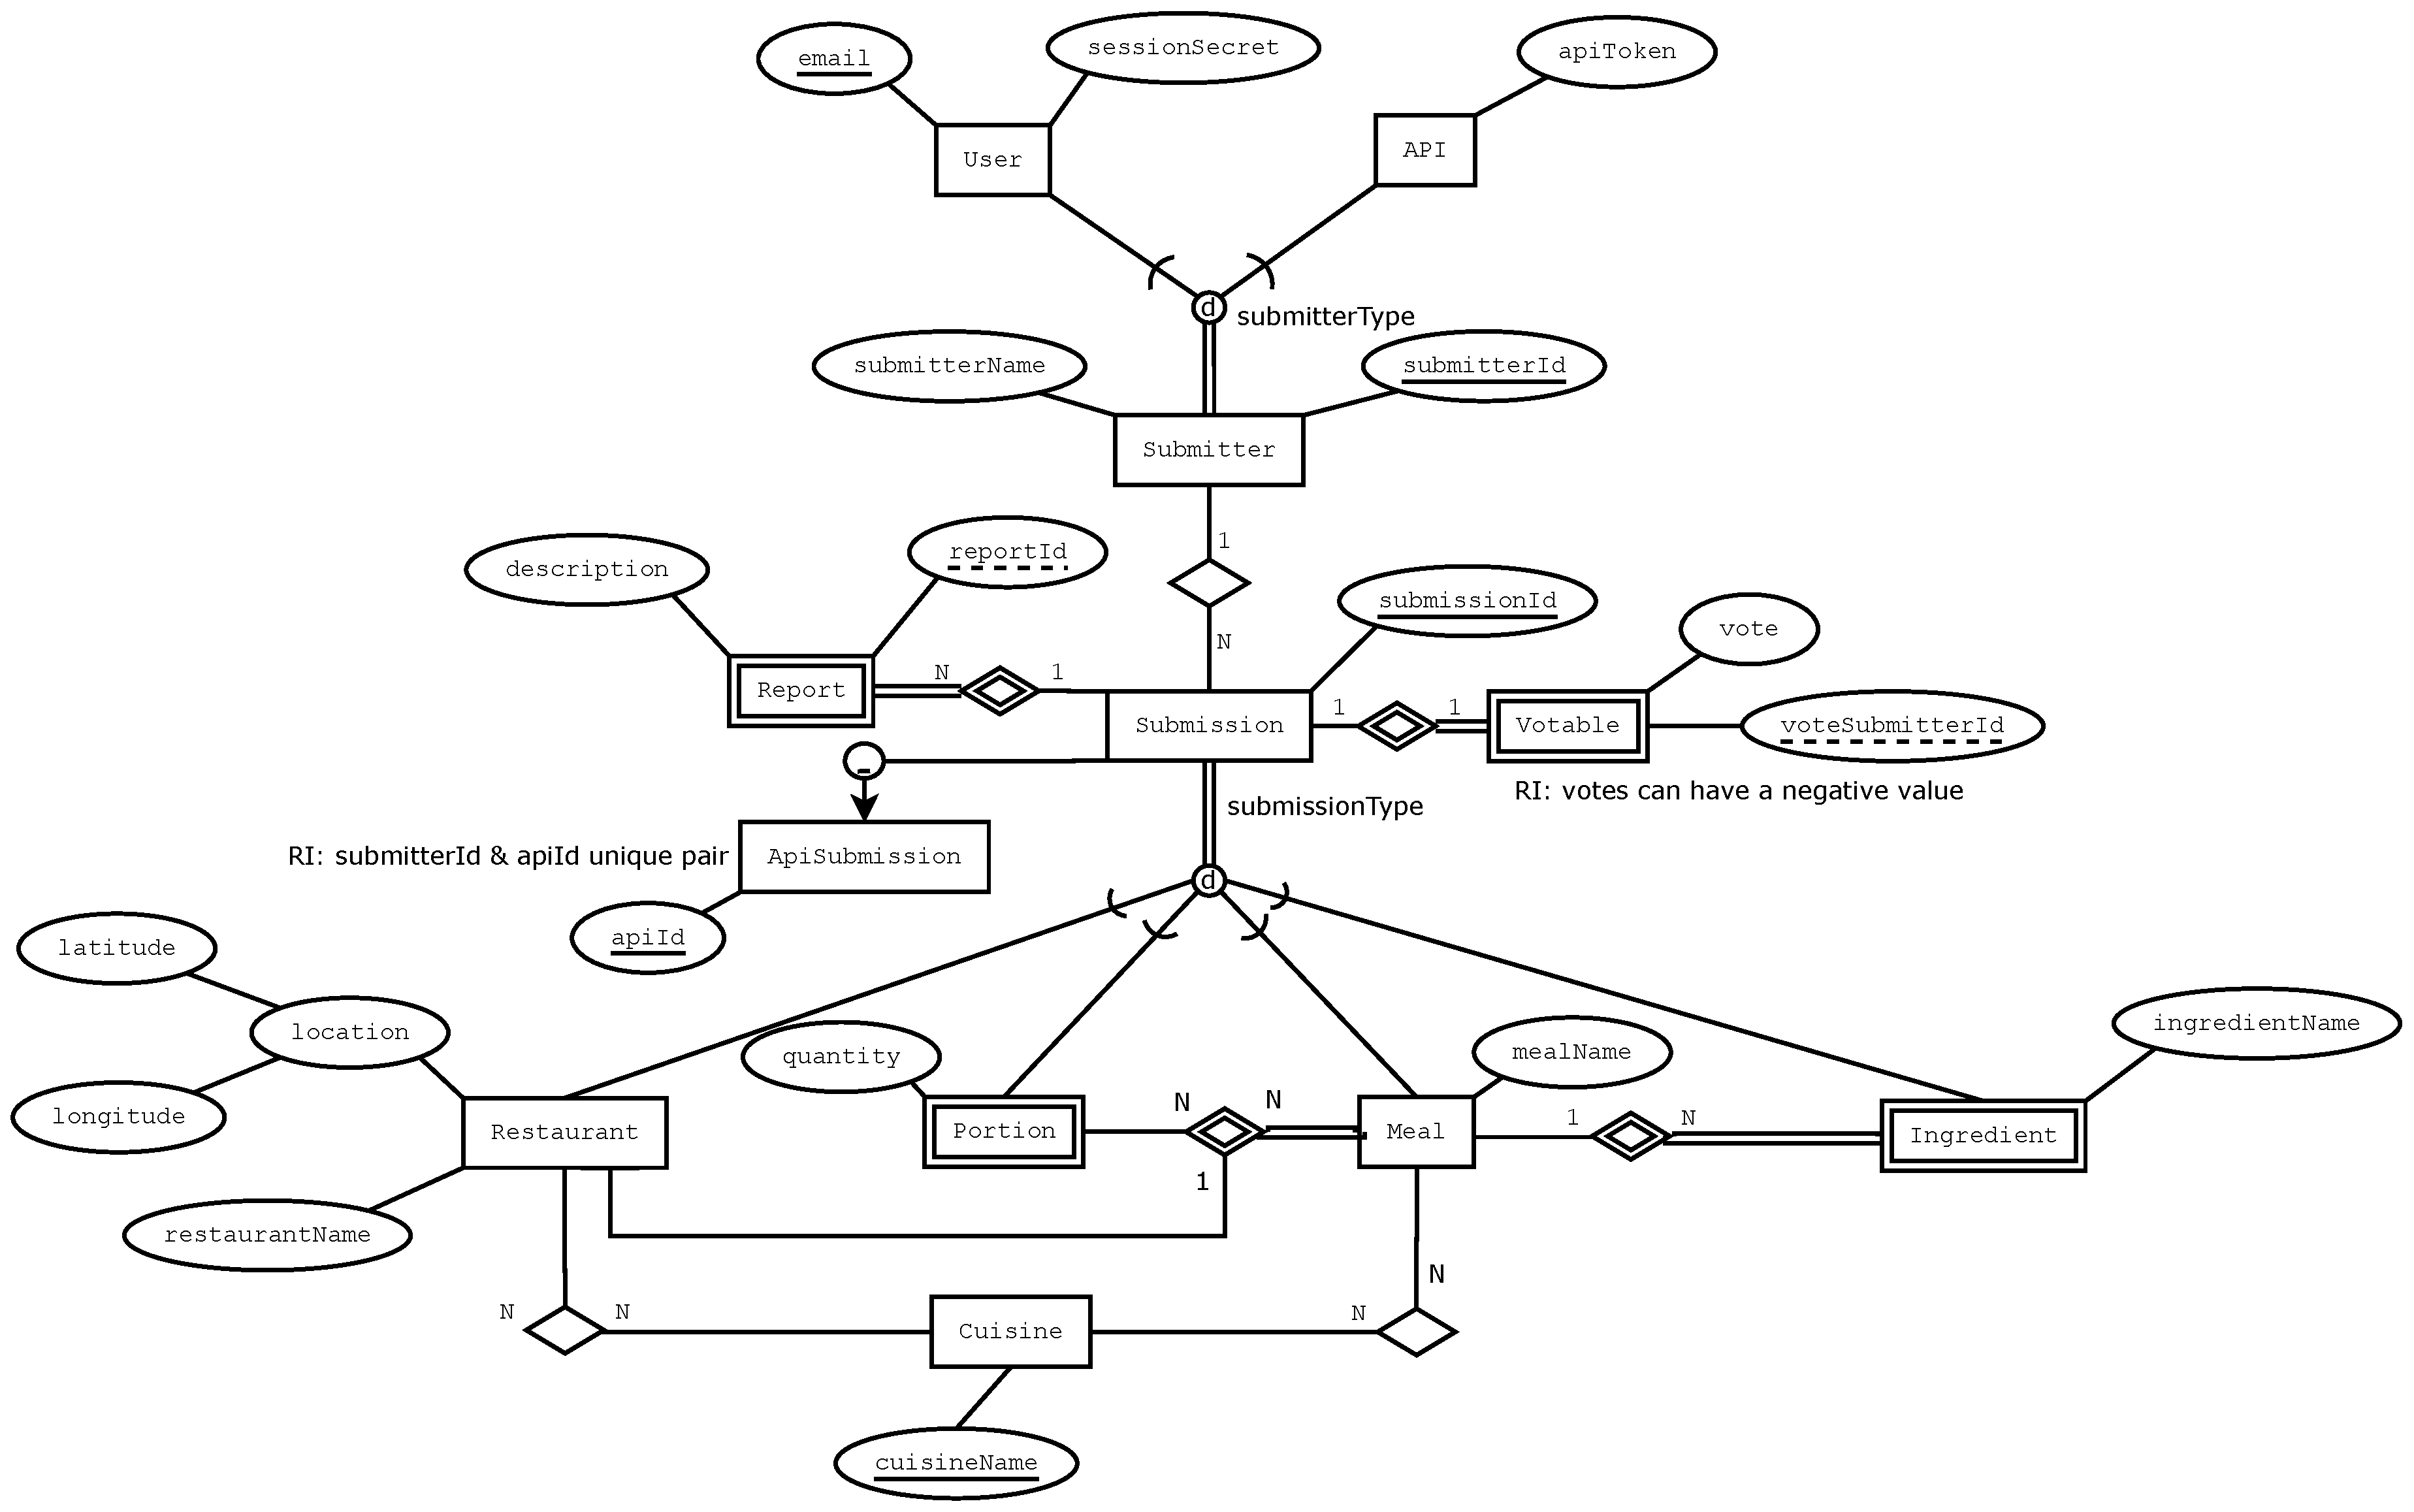
\includegraphics[scale=0.28]{Nutr.io_Database_Diagram.eps}
    \centering 
\end{figure}
\newpage

\section{Normalized Relational Model}
    \begin{itemize}
        \item \textbf{Submitter}        
        \begin{itemize}
            \item Attributes: \underline{submitterId}, submitterName, submitterType
            \item Primary Key(s): \underline{submitterId}
            \item Foreign Key(s): -
            \item Not null: submitterName, submitterType
        \end{itemize}

        \item \textbf{User}
        \begin{itemize}
            \item Attributes: \underline{\textit{submitterId}}, \underline{email}, sessionSecret
            \item Primary Key(s): \underline{\textit{submitterId}}, \underline{email}
            \item Foreign Key(s): \underline{\textit{submitterId}} references Submitter(submitterId)
            \item Not null: sessionSecret
        \end{itemize}

        \item \textbf{API}
        \begin{itemize}
            \item Attributes: \underline{\textit{submitterId}}, apiToken
            \item Primary Key(s): \underline{\textit{submitterId}}
            \item Foreign Key(s): \underline{\textit{submitterId}} references Submitter(submitterId)
            \item Not null: apiToken
        \end{itemize}

        \item \textbf{Submission}
        \begin{itemize}
            \item Attributes: \underline{submissionId}, submissionType
            \item Primary Key(s): \underline{submissionId}            
            \item Not null: submissionType
        \end{itemize}

        \item \textbf{ApiSubmission}
        \begin{itemize}
            \item Attributes: \underline{\textit{submissionId}}, \underline{apiId}, submissionType
            \item Primary Key(s): \underline{\textit{submissionId}}, \underline{apiId}
            \item Foreign Key(s): \underline{\textit{submissionId}} references Submission(submissionId)
            \item Not null: submissionType
        \end{itemize}

        \item \textbf{SubmissionSubmitter}
        \begin{itemize}
            \item Attributes: \underline{\textit{submissionId}}, \underline{\textit{submitterId}}, submissionDate
            \item Primary Key(s): \underline{\textit{submissionId}}, \underline{\textit{submitterId}}
            \item Foreign Key(s): 
            \begin{itemize}
                \item \underline{\textit{submissionId}} references Submission(submissionId)
                \item \textit{submitterId} references Submitter(submitterId)
            \end{itemize}
            \item Not null: \textit{submitterId}
        \end{itemize}

        \item \textbf{SubmissionContract}
        \begin{itemize}
            \item Attributes: \underline{submissionId}, \underline{submissionContract}
            \item Primary Key(s): \underline{submissionId}, \underline{submissionContract}
        \end{itemize}

        \item \textbf{Report}
        \begin{itemize}
            \item Attributes: \underline{\textit{submitterId}}, \underline{\textit{submissionId}}, description
            \item Primary Key(s): \underline{\textit{submitterId}}, \underline{\textit{submissionId}}
            \item Foreign Key(s): 
            \begin{itemize}
                \item \underline{\textit{submissionId}} references Submission(submissionId)
                \item \underline{\textit{submitterId}} references Submitter(submitterId)
            \end{itemize}
            \item Not null: description
        \end{itemize}

        \item \textbf{Vote}
        \begin{itemize}
            \item Attributes: \underline{\textit{submissionId}}, \underline{\textit{voteSubmitterId}}, vote
            \item Primary Key(s): \underline{\textit{voteSubmitterId}}, \underline{\textit{submissionId}}
            \item Foreign Key(s): 
                \begin{itemize}
                    \item \underline{\textit{submissionId}} references Submission(submissionId)
                    \item \underline{\textit{voteSubmitterId}} references Submitter(submitterId)
                \end{itemize}
            \item Not null: vote
        \end{itemize}

        \item \textbf{Restaurant}
        \begin{itemize}
            \item Attributes: \underline{\textit{submissionId}}, restaurantName, latitude, longitude
            \item Primary Key(s): \underline{\textit{submissionId}}
            \item Foreign Key(s): \underline{\textit{submissionId}} references Submission(submissionId)
            \item Not null: restaurantName
        \end{itemize}
    
        \item \textbf{Cuisine}
        \begin{itemize}
            \item Attributes: \underline{cuisineName}
            \item Primary Key(s): \underline{cuisineName}        
        \end{itemize}

        \item \textbf{Meal}
        \begin{itemize}
            \item Attributes: \underline{\textit{submissionId}}, mealName
            \item Primary Key(s): \underline{\textit{submissionId}}
            \item Foreign Key(s): \underline{\textit{submissionId}} references Submission(submissionId)
            \item Not null: mealName
        \end{itemize}

        \item \textbf{Portion}
        \begin{itemize}
            \item Attributes: \underline{\textit{submissionId}}, quantity
            \item Primary Key(s): \underline{\textit{submissionId}}
            \item Foreign Key(s): \underline{\textit{submissionId}} references Submission(submissionId)
            \item Not null: quantity
        \end{itemize}

        \item \textbf{Ingredient}
        \begin{itemize}
            \item Attributes: \underline{\textit{submissionId}}, ingredientName
            \item Primary Key(s): \underline{\textit{submissionId}}
            \item Foreign Key(s): \underline{\textit{submissionId}} references Submission(submissionId)
            \item Not null: ingredientName
        \end{itemize}

        \item \textbf{MealIngredient}
        \begin{itemize}
            \item Attributes: \underline{\textit{mealSubmissionId}}, \underline{\textit{ingredientSubmissionId}}
            \item Primary Key(s): \underline{\textit{mealSubmissionId}}, \underline{\textit{ingredientSubmissionId}}
            \item Foreign Key(s): 
                \begin{itemize}
                    \item \underline{\textit{mealSubmissionId}} references Meal(submissionId)
                    \item \underline{\textit{ingredientSubmissionId}} references Ingredient(submissionId)
                \end{itemize}   
        \end{itemize}

        \item \textbf{RestaurantMealPortion}
        \begin{itemize}
            \item Attributes: \underline{\textit{mealSubmissionId}}, \underline{\textit{portionSubmissionId}}, \textit{restaurantSubmissionId}
            \item Primary Key(s): \underline{\textit{mealSubmissionId}}, \underline{\textit{portionSubmissionId}}
            \item Foreign Key(s):
            \begin{itemize}
                \item \underline{\textit{mealSubmissionId}} references Meal(submissionId)
                \item \underline{\textit{portionSubmissionId}} references Portion(submissionId)
                \item \textit{restaurantSubmissionId} references Restaurant(submissionId)
            \end{itemize}            
        \end{itemize}

        \item \textbf{RestaurantCuisine}
        \begin{itemize}
            \item Attributes: \underline{\textit{restaurantSubmissionId}}, \underline{\textit{cuisineName}}
            \item Primary Key(s): \underline{\textit{restaurantSubmissionId}}, \underline{\textit{cuisineName}}
            \item Foreign Key(s): 
                \begin{itemize}
                    \item \underline{\textit{restaurantSubmissionId}} references Restaurant(submissionId)
                    \item \underline{\textit{cuisineName}} references Cuisine(cuisineName)
                \end{itemize}   
        \end{itemize}

        \item \textbf{MealCuisine}
        \begin{itemize}
            \item Attributes: \underline{\textit{mealSubmissionId}}, \underline{\textit{cuisineName}}
            \item Primary Key(s): \underline{\textit{mealSubmissionId}}, \underline{\textit{cuisineName}}
            \item Foreign Key(s): 
                \begin{itemize}
                    \item \underline{\textit{mealSubmissionId}} references Meal(submissionId)
                    \item \underline{\textit{cuisineName}} references Cuisine(cuisineName)
                \end{itemize}   
        \end{itemize}
    \end{itemize}
\end{document}